
\chapter{Исследование модельного порыва}


В прямых трубах круглого сечения, как и в некоторых других сдвиговых течениях, переход к турбулентности может происходить без потери ламинарным течением линейной устойчивости. В частности, в приведенной в разделе \ref{math_section} постановке ламинарное течение (течение Пуазейля в круглой трубе) линейно устойчиво при всех числах Рейнольдса \cite{Kerswell2005}. Для выхода на турбулентный режим течения необходимо внести в поток возмущения достаточно большой амплитуды, в то время как малые возмущения ламинарного течения затухают. В таких условиях существуют возмущения некоторой критической амплитуды, отделяющие возмущения, вызывающие переход к турбулентности, от затухающих. В фазовом пространстве соответствующие критическим возмущениям решения принадлежат сепаратрисе, разделяющей области притяжения решений, соответствующих ламинарному и турбулентному режимам течения. Принадлежащее в первый момент времени сепаратрисе решение остается на сепаратрисе. Хотя решение, эволюционирующее на сепаратрисе, неустойчиво и не может наблюдаться в эксперименте, оно может быть получено численно. Замечено, что решение на сепаратрисе сохраняет некоторое характерные черты турбулентного течения, но при этом имеет более простую форму и динамику. 

Метод поиска решения на сепаратрисе предложен в работе \cite{Skufca2006}. Первые расчеты решения на сепаратрисе в круглой трубе выполнены в расчетной области небольшой протяженности (с условием периодичности вдоль потока) \cite{Schneider2007}. В расчетах \cite{Mellibovsky2009transition, Duguet2010}, выполненных в протяженной расчетной области, обнаружено, что при переходных числах Рейнольдса решение на сепаратрисе в круглой трубе имеет пространственно локализованную структуру. При этом, если турбулентность существует в форме пространственно локализованных порывов до $\Re \approx 2700$, то решение на сепаратрисе имеет пространственно локализованную структуру по крайней мере до $\Re = 6000$. С ростом числа Рейнольдса амплитуда отклонения от ламинарного течения и протяженность области локализации в решении на сепаратрисе снижаются \cite{Duguet2010}, что дает основание полагать, что решение на сепаратрисе сохраняет локализованную структуру и при больших числах Рейнольдса (хотя расчеты при больших $\Re$ не проводились). Как отмечено в \cite{Duguet2010, Avila2013}, решение на сепаратрисе в круглой трубе воспроизводит ряд характерных особенностей турбулентного порыва, и при небольших значениях числа Рейнольдса их характеристики оказываются близки друг к другу. Структуры, напоминающие локализованное решение на сепаратрисе, наблюдались в экспериментах \cite{deLozar2012} и в численных расчетах \cite{Manneville2011} при затухании турбулентного течения. 
% Расчеты решения на сепаратрисе в плоском течении Куэтта \cite{Schneider2008}
% Решение на сепаратрисе в плоском течении Куэтта в протяженной расчетной области имеет локализованную структуру \cite{Duguet2009}

В работе \cite{Avila2013} обнаружено, что при наложении на решение, описывающее течение в круглой трубе, дополнительных условий симметрии при переходном значении числа Рейнольдса решение, эволюционирующее на сепаратрисе, приближается к условно периодическому решению. Предельное решение сохраняет пространственно локализованную структуру, но в сопутствующей системе отсчета оказывается периодическим по времени. Помимо пространственной локализации предельное решение воспроизводит некоторые другие характерные особенности турбулентного порыва (см. раздел \ref{edge_char_seq}). Мы будем называть это решение {\it модельным порывом}. Простота поведения модельного порыва позволяет выполнить его подробное исследование, что может помочь прояснить свойства турбулентного порыва. 

В главе представлен метод получения модельного порыва, описаны его основные характеристики и внутренняя структура; даны оценки достоверности полученных результатов. Детальное описание внутренней структуры модельного порыва выполнено автором диссертации и является новым научным результатом. Основные результаты, приведенные в этом разделе, опубликованы в работах автора диссертации \cite{MZG2015, Kazan2015, KMU2014, KMU2015}. 

\section{Расчет модельного порыва} \label{edge_seq}

Следуя \cite{Avila2013}, решение поставленной в разделе \ref{math_section} задачи ищется с дополнительными ограничениями диаметральной симметричности и $\pi$-периодичности в угловом направлении:
\begin{equation}\label{sym_eq}
(v_x, v_r, v_\theta)(x, r, -\theta, t) = (v_x, v_r, -v_\theta)(x, r, \theta, t),
\end{equation}
\begin{equation}\label{per_eq}
(v_x, v_r, v_\theta)(x, r, \theta+\pi, t) = (v_x, v_r, v_\theta)(x, r, \theta, t).
\end{equation}
Здесь $(x, r, \theta)$ --- цилиндрические координаты, $(v_x, v_r, v_\theta)$ --- продольная, радиальная и угловая компоненты вектора скорости. Наложение ограничений \eqref{sym_eq}, \eqref{per_eq} упрощает поведение решения в пространстве, делает его более определенным. Условие \eqref{sym_eq} ограничивает возможность смещения турбулентных структур в угловом направлении.  Турбулентные порывы, рассчитанные при $Re=2000$ с учетом и без учета условий \eqref{sym_eq}, \eqref{per_eq} изображены на Рисунке~\ref{3D_img} (представлены области пониженной и повышенной на $0.1$ скорости относительно течения Пуазейля). В обоих случаях порыв имеет центральное ядро с пониженной скоростью и систему вытянутых вдоль стенки трубы, чередующихся в угловом направлении полос замедления и ускорения. На симметричном порыве полосы гораздо более структурированы. Их угловое положение не меняется в процессе эволюции: угловые области $\theta=k\pi/2$, $k$ от $0$ до $3$, где в силу \eqref{sym_eq}, \eqref{per_eq} угловая компонента скорости тождественно равна нулю, заняты полосами ускорения, промежуточные области $\theta=\pi/4+k\pi/2$ --- полосами замедления. На порыве без условий симметрии наблюдаются значительные по амплитуде случайные по пространственному расположению флуктуации, разрывающие сплошность полосчатых структур. На симметричном порыве тоже заметна флуктуирующая компонента, которая в этом случае выглядит гораздо более регулярной. Отметим, что несмотря на заметную пространственную регулярность, временн\'{о}е поведение симметричного порыва остается хаотичным.


\begin{figure}[h]
\center{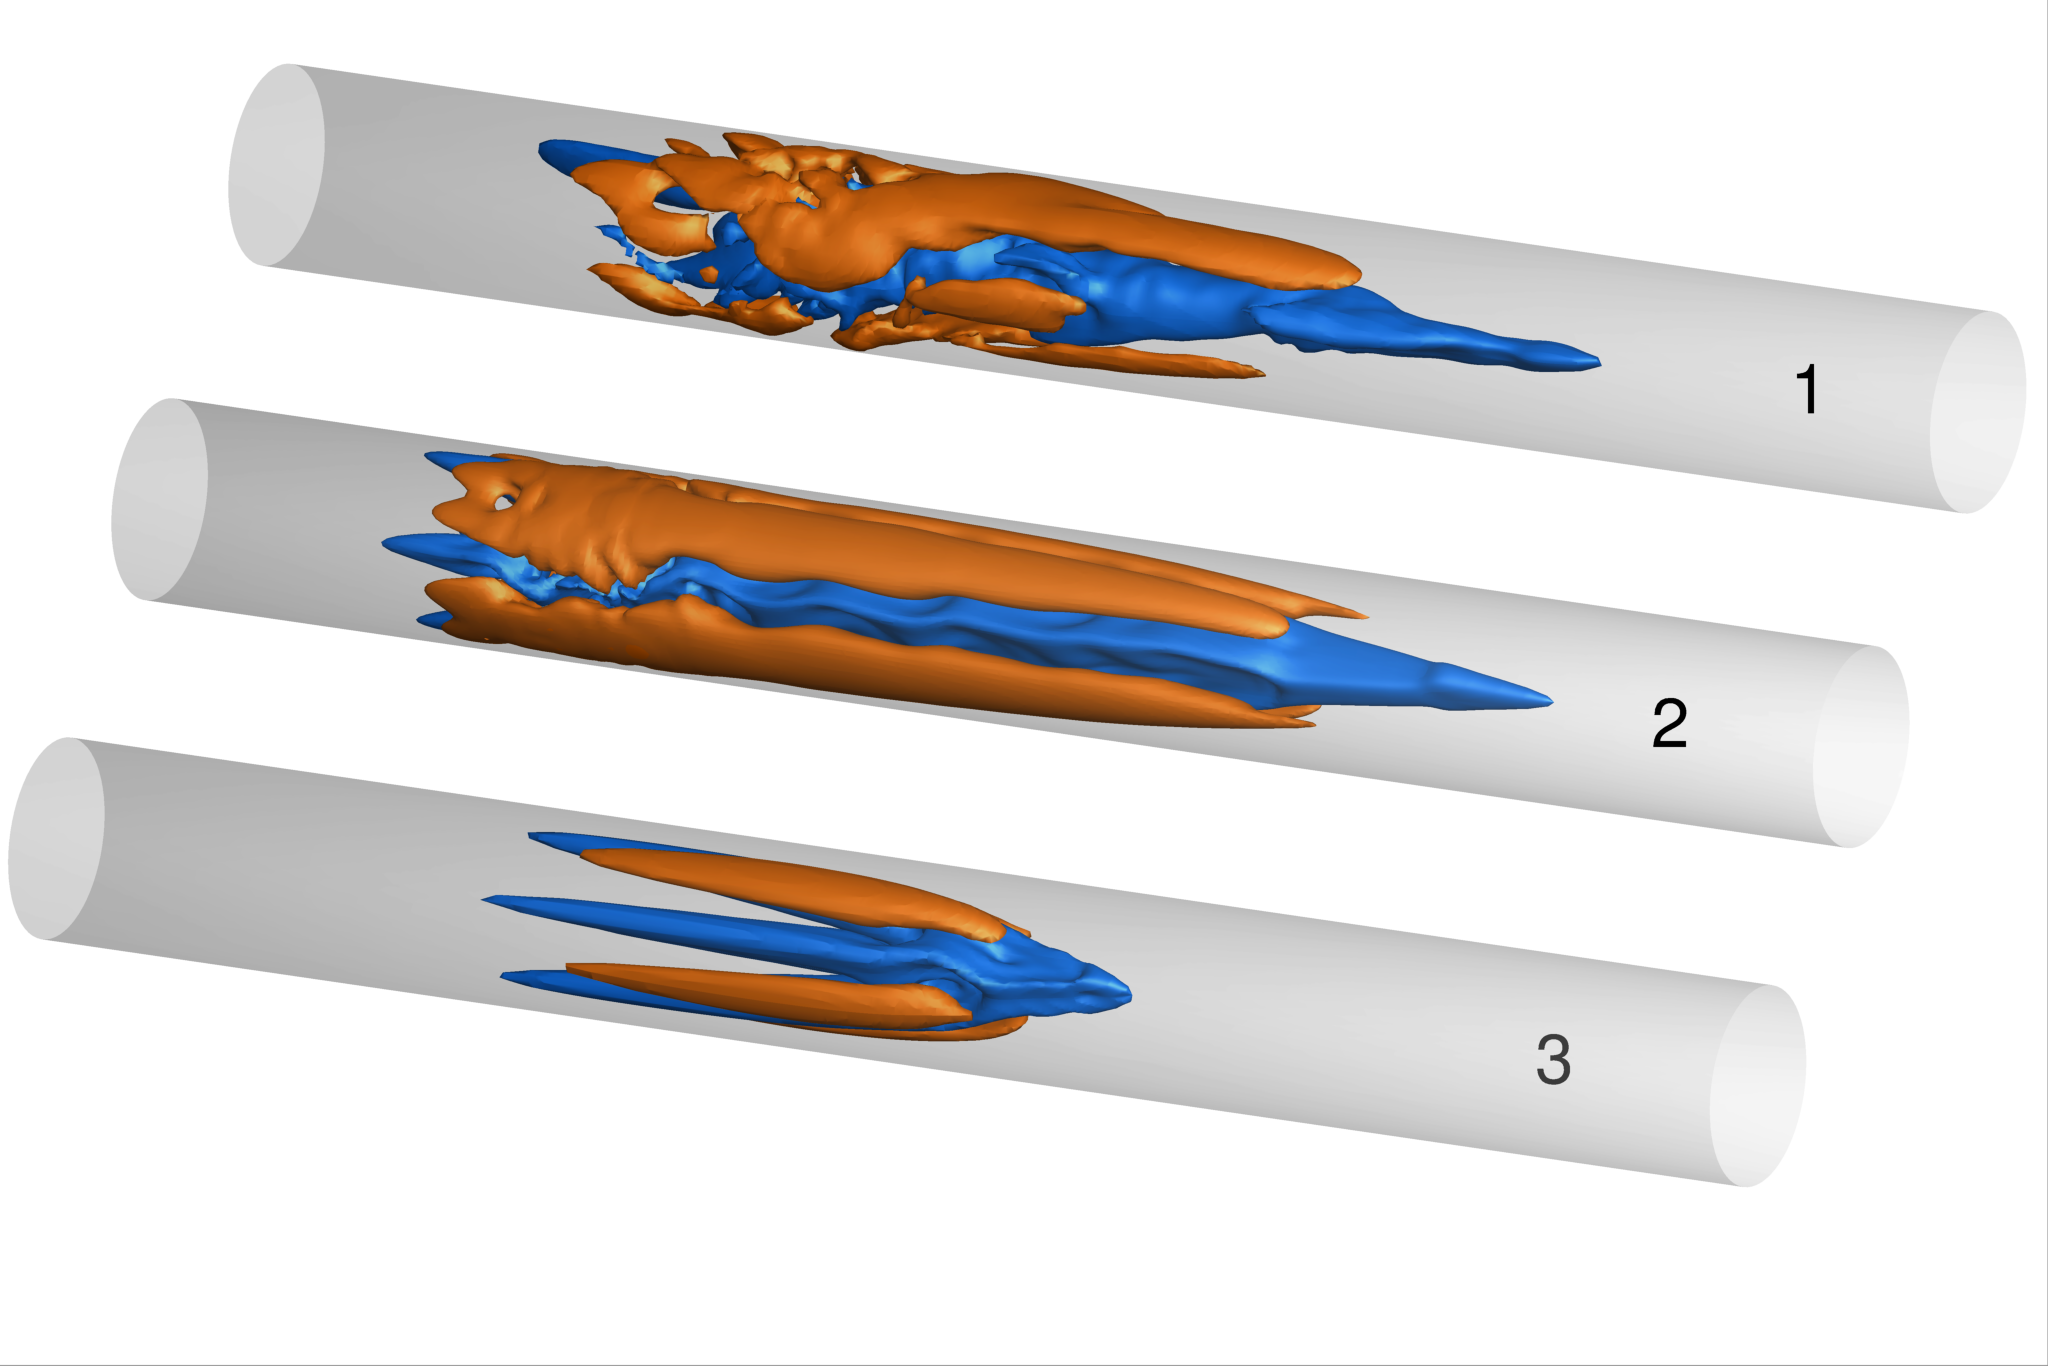
\includegraphics[width=1\linewidth]{3D_cmp.png}}
\caption{Визуализация численных расчетов турбулентных порывов: 1 --- $\Re = 2000$; 2 --- $\Re = 2000$ с учетом \eqref{sym_eq}, \eqref{per_eq}; 3 --- решение на сепаратрисе, $\Re = 2200$. Темным и светлым тоном выделены поверхности скорости $-0.1$ и $+0.1$ относительно скорости течения Пуазейля. Поток направлен слева направо.}
\label{3D_img}
\end{figure}

Предельное решение на сепаратрисе получено при $\Re=2200$. Условие \eqref{per_eq} при \eqref{sym_eq} порождает условие отражения относительно сечения $\theta = \pi/2$, аналогичное условию отражения относительно сечения $\theta = 0$:
\begin{equation} \label{sym2_eq}
(v_x, v_r, v_\theta)(x, r, \pi/2 + \theta, t) = (v_x, v_r, -v_\theta)(x, r, \pi / 2 - \theta, t).
\end{equation}
С учетом \eqref{sym_eq}, \eqref{sym2_eq} расчет проводился для четверти объема трубы $0\leqslant\theta\leqslant\pi/2$. Исходное решение найдено при $L_x = 80$ на сетке, содержащей $512 \times 32 \times  32$ ячеек в продольном, радиальном и угловом направлениях. 

Предварительно найденное турбулентное решение $\v_{turb}(\x,t)$ используется в итерационной процедуре отыскания предельного решения на сепаратрисе. Задача решается с начальным условием
\begin{equation} \label{edge_init_eq}
\v(\x,t=0) = \v_{Pois}(\x)+\alpha(\v_{turb}(\x,t=t_0) - \v_{Pois}(\x)).
\end{equation}
Здесь $\v_{Pois}=(1-r^2,0,0)$ --- течение Пуазейля, $t_0$ --- некоторый фиксированный момент времени, $\alpha \in [0,1]$ --- скалярный параметр. Значение $\alpha=0$ соответствует нулевому возмущению, и решением при $t > 0$ остается течение Пуазейля. Выбирая $\alpha=1$, уже в начальный момент времени реализуется турбулентный режим, который сохраняется при $t > 0$. При промежуточных значениях $\alpha$ происходит стремление решения либо к одному, либо к другому режиму. Применяя метод деления пополам, мы постепенно отыскиваем то значение $\alpha$, при котором решение эволюционирует на сепаратрисе, разделяющей области притяжения двух режимов течения. Суть метода состоит в том, что если при текущем значении $\alpha$ возмущения затухают, то на следующей итерации $\alpha$ увеличивается; если развивается турбулентный режим течения --- $\alpha$ уменьшается. На Рисунке \ref{bisection_pic} представлены графики $A(t)$ – среднеквадратичного по всему объему отклонения поля скорости от течения Пуазейля для нескольких значений $\alpha$, демонстрирующие сходимость итерационного процесса. При уточнении значения $\alpha$ продлевается длительность балансирования решения на сепаратрисе.


\begin{figure}
\center{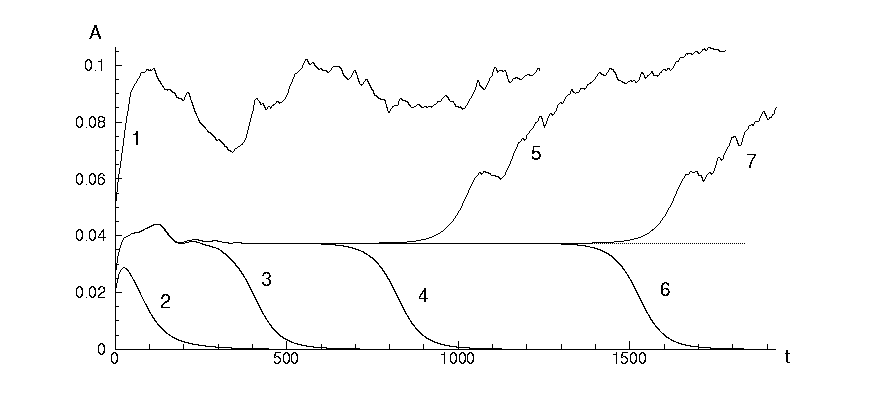
\includegraphics[width=1\linewidth]{bisection.png}}
\caption{Итерационный процесс построения решения на сепаратрисе. 1--7 --- эволюция среднеквадратичной амплитуды возмущений $A(t)$ при уточнении значения $\alpha$.}
\label{bisection_pic}
\end{figure}

С каждой новой итерацией решение проводит на сепаратрисе в среднем на 30 единиц времени больше. В расчетах для представления действительных числе использованы 64-битные числа с плавающей запятой. Это позволило найти около 50 приближений к решению на сепаратрисе. Соответственно, решение удалось удержать на сепаратрисе в течении приблизительно 1500 единиц времени. Из них ориентировочно первые 500 единиц происходит перестройка решения, после чего режим течения устанавливается. В согласии с результатами \cite{Avila2013}, решение на сепаратрисе при $\Re=2200$ постепенно выходит на условно периодический режим. Это решение описывает локализованной в пространстве структуры, которая сносится вниз по потоку с постоянной скоростью. В подвижной системе отсчета поле скорости в каждой точке испытывает периодические колебания. Для скорости сноса и периода колебаний получены значения $c=0.69$ и $T=60$ (в \cite{Avila2013} сообщается о $c=0.76$ и $T=60$). Во всех выполненных расчетах режим течения, устанавливающийся на сепаратрисе, не зависит от исходного турбулентного поля скорости $\v_{turb}$. 

\begin{comment}
Так как скорость сноса модельного порыва заранее не известна, решение на сепаратрисе было найдено в системе отсчета, двигающейся со скоростью $0.5$. После того, как решение на сепаратрисе найдено, изменить скорость перемещения системы отсчета уже не представляется возможным вследствие высокой чувствительности решения к возмущениям, возникающим в данном случае в результате неточностей численного интегрирования. Чтобы получить решение в сопутствующей системе отсчета, метод поиска решения на сепаратрисе применен повторно в системе отсчета, двигающейся с уже известной скоростью перемещения порыва. 
\end{comment}

Сравнение предельного решения на сепаратрисе с турбулентным порывом, представленное на Рисунке \ref{3D_img}, показывает качественное согласие этих решений. Во всех структурах имеются протяженные области ускоренного и замедленного движения, концентрирующиеся в пристенной области трубы. Сохраняется и основная качественная особенность порыва --- медленное понижение осевой скорости на его передней границе и более резкое восстановление скорости на задней границе (смотри Рисунок \ref{ucl_cmp_img}). Мы будем называть предельное решение на сепаратрисе {\it модельным порывом}.  

\begin{figure}
\center{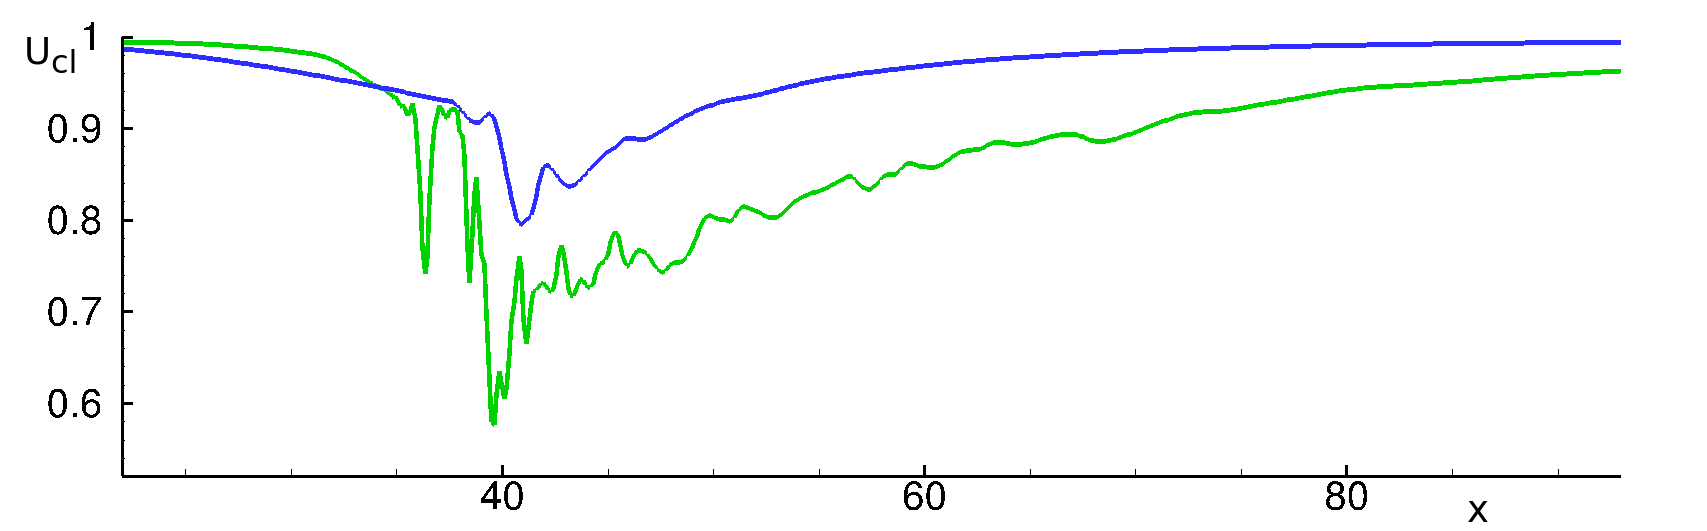
\includegraphics[width=0.7\linewidth]{ucl_cmp.png}}
\caption{Сравнение скорости на оси трубы в турбулентном (1) и модельном (2) порывах.}
\label{ucl_cmp_img}
\end{figure}

Для того, чтобы установить влияние условия периодичности вдоль трубы на предельное решение, решение было найдено в расчетной области вдвое большей протяженности, при $L_x = 160$ (число узлов сетки в продольном направлении также удвоено). Также при исходном значении $L_x = 80$ решение было получено на более подробной сетке, содержащей $1024 \times 64 \times 64$ ячеек (в сравнении с исходной сеткой в каждом направлении число ячеек удвоено). Результаты, полученные на трех сетках, качественно совпадают и количественно близки. Для сравнения, на Рисунке \ref{amp_pic} представлены некоторые интегральные характеристики модельного порыва, полученные на различных сетках (подробное описание изображенных величин приведено в следующем разделе). Полученные результаты подтверждают достаточность расчетной сетки и длины расчетной области для адекватного воспроизведения модельного порыва, а также то, что его пространственная локализация не связана с условием периодичности вдоль трубы. Характеристики полученного модельного порыва согласуются с результатами работы \cite{Avila2013}. Это подтверждает, что найденное решение является решением математической задачи и не зависит от численного метода, которым оно было найдено. В работе \cite{Avila2013} решение получено двумя методами --- полностью спектральным \cite{Meseguer2007} и спектрально-конечно-разностным \cite{Willis2009}. Мы применяем конечно-разностный метод \cite{Nikitin2006}. Также, модельный порыв был воспроизведен в работе \cite{Chantry2014} спектрально-конечно-разностным методом \cite{Willis2009}; авторами также сообщается о совпадении результатов с \cite{Avila2013}. 


\section{Основные свойства модельного порыва} \label{edge_char_seq}

При $\Re=2200$ модельный порыв имеет длину около $40R$ и перемещается вдоль трубы со скоростью $c = 0.69U$. В подвижной системе отсчета он является периодическим по времени с периодом $T = 60 R/U$. Характерным свойством модельного порыва является наличие вытянутых вдоль потока областей с повышенным и пониженным значением продольной компоненты скорости, чередующихся в угловом направлении (смотри Рисунок \ref{3D_img}). Полосы повышенной скорости целиком расположены около стенки трубы, полосы замедления соединяются в единое целое в приосевой области вблизи переднего фронта. Наличие вытянутых вдоль потока полос ускоренного и замедленного движения --- характерное свойство любого пристенного турбулентного течения. Однако, в отличие от реальной турбулентности, где полосы случайно блуждают во времени и в пространстве, в рассматриваемом решении полосы сохраняют свое положение и форму, лишь слегка искажаясь периодическими колебаниями. 

\begin{figure}
\center{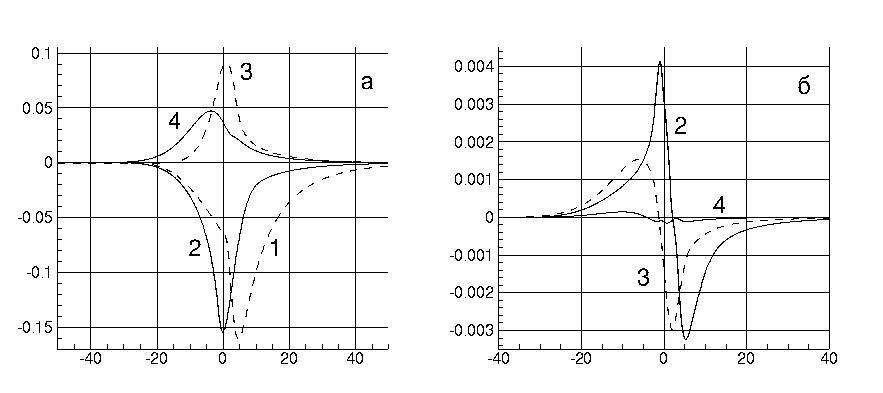
\includegraphics[width=1\linewidth]{U2D.png}}
\caption{Распределения вдоль трубы продольной (a) и радиальной (b) компоненты осесимметричной составляющей скорости $\V_{2D}$ для нескольких расстояний от оси трубы: 1–4 – r = 0, 0.4, 0.7, 0.9}
\label{U2D_pic}
\end{figure}

Для удобства перейдем в подвижную систему координат, перемещающуюся вдоль трубы со скоростью сноса локализованной структуры. В подвижной системе решение представляется в виде суперпозиции стационарной составляющей $\V(\x) = \overline{\v}^t$ и колебательной $\v_n(t,\x) = \v - \V$. Стационарную составляющую, в свою очередь, представим в виде суперпозиции осесимметричной $\V_{2D}(\x) = \overline{\V}^{\theta}$ и трехмерной $\V_{3D}(\x) = \V - \V_{2D}$ составляющих. Распределения продольной компоненты осесимметричной составляющей скорости вдоль трубы $V_{x,2D}(x)$ для нескольких расстояний от оси трубы представлены на Рисунке \ref{U2D_pic}(а) (даны отклонения от течения Пуазейля). Начало системы отсчета $x=0$ помещено в сечение, в котором среднее отклонение скорости от течения Пуазейля максимально. Голова структуры, где начинает проявляться отклонение осевой скорости, располагается на расстоянии $x \approx 45$. Хвостовая часть структуры на сепаратрисе очерчена не так четко, как в турбулентных порывах, где восстановление скорости происходит на отрезке длиной в $3-5$ радиусов трубы.  Падение скорости в приосевой области трубы компенсируется ускорением у стенки. Поведение радиальной компоненты $V_{r,2D}$, показанное на Рисунке \ref{U2D_pic}(b), соответствует изменению осевой скорости --- в зоне замедления на оси происходит растекание жидкости к стенкам, $V_{r,2D}>0$, в передней части происходит обратный процесс и $V_{r,2D}<0$.

\begin{figure}
\center{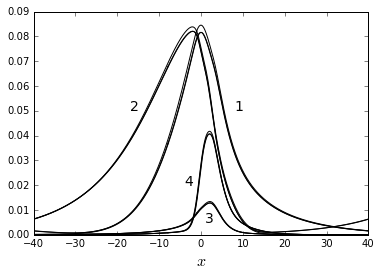
\includegraphics[width=0.6\linewidth]{amp.png}}
\caption{Распределения вдоль трубы среднеквадратичных по сечению амплитуд трех составляющих движения: 1 -- $\V_{2D}$ (отклонение от течения Пуазейля); 2, 3 -- продольная и поперечные компоненты скорости $\V_{3D}$; 4 -- $\v_{n}$. Представлены результаты, полученные на трех расчетных сетках, параметры которых приведены в разделе \ref{edge_seq}. }
\label{amp_pic}
\end{figure}

На Рисунке \ref{amp_pic} приведены распределения по $x$ среднеквадратичных по сечению трубы амплитуд трех составляющих движения: стационарной осесимметричной (отклонение от течения Пуазейля) $A_{2D}$, стационарной трехмерной $A_{3D}$ и колебательной $A_n$. Распределение $A_{2D}(x)$ соответствует Рисунку \ref{U2D_pic}. Отклонение от течения Пуазейля заметно на значительном отрезке от $x=-30$ до $x=40$. Максимум $A_{2D}$ составляет 8.4\%. Величина $A_{3D}$ характеризует интенсивность полосчатых структур. Как видно на Рисунке~\ref{3D_img}, полосчатые структуры появляются на некотором расстоянии вверх по потоку от головы порыва и сохраняются на значительном расстоянии позади него. В соответствии с этим $A_{3D}(x)$ имеет выраженную асимметрию относительно точки $x=-2$, где эта величина достигает максимума. Интенсивность полос быстро падает вниз по потоку и сохраняется на значительном расстоянии в верхней части потока. В отличие от стационарных полосчатых структур, колебательная составляющая движения сосредоточена на сравнительно непротяженном отрезке трубы от $x=-5$ до $x=15$ с максимальной амплитудой в 4\% при $x=2.5$.


\begin{figure}[h]
\center{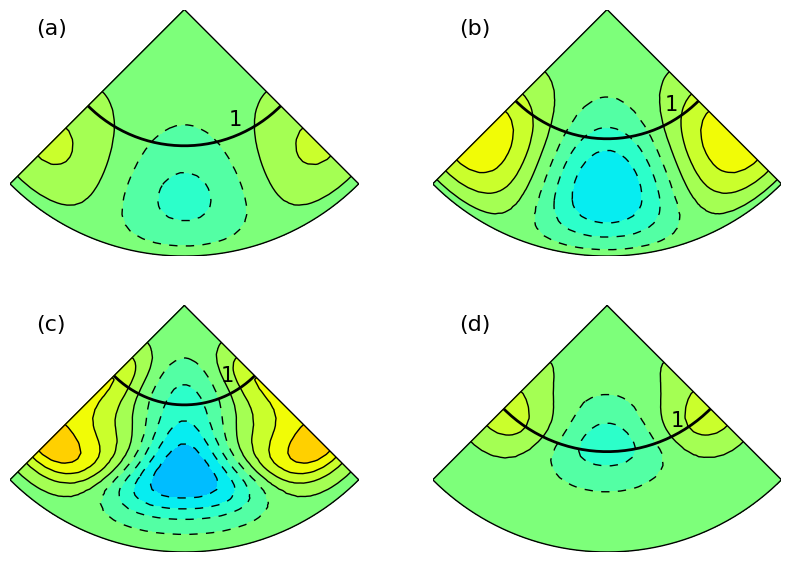
\includegraphics[width=0.8\linewidth]{V3D_cs.png}}
\caption{Значение $V_{x,3D}$ в нескольких сечениях трубы: (a)--(d) --- $x = -20, -10, 0, 5$. Изолинии построены с шагом $\approx 0.04$. Сплошные линии --- положительные значения, прерывистые --- отрицательные значения. На линии~1 относительная скорость жидкости равна нулю ($V_{x} = c$). }
% d = 0.0429
\label{V3D_cs_pic}
\end{figure}


В трехмерную стационарную составляющую движения $\V_{3D}$ попадают полосы повышенной и пониженной скорости. Поле $V_{x,3D}$ в нескольких сечениях трубы изображено на Рисунке~\ref{V3D_cs_pic}. В каждом сечении трубы полосы пониженной скорости ($V_{x,3D} < 0$) проходят через центр расчетной области, при $\theta = \pi/4$. Полосы повышенной скорости ($V_{x,3D} > 0$) попадают на границы расчетной области в угловом направлении, находящиеся при $\theta = 0, \pi/2$. Среднее поле скорости оказывается симметрично относительно плоскости, проходящей через центр расчетной области при $\theta = \pi/4$, так как поле скорости решения на сепаратрисе $\v = (v_x, v_r, v_\theta)$ имеет дополнительную симметрию отражения относительно указанной плоскости со сдвигом на половину периода по времени:
\begin{equation}
(v_x, v_r, v_\theta)(x, r, \pi/4 + \theta, t) = (v_x, v_r, -v_\theta)(x, r, \pi/4 - \theta, t + T/2). 
\end{equation} 


\begin{figure}[h]
\center{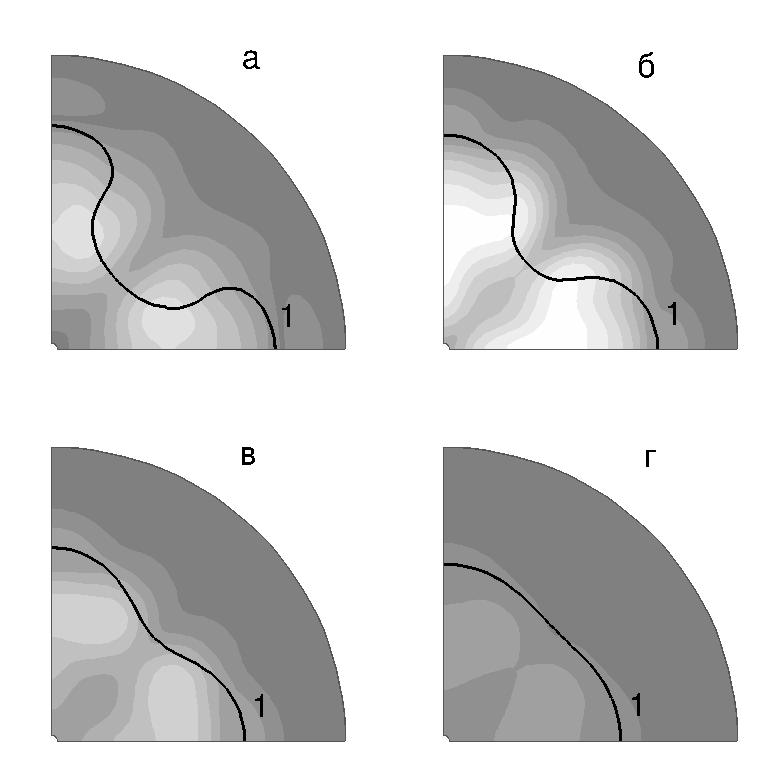
\includegraphics[width=0.8\linewidth]{puls_cs.png}}
\caption{Изолинии среднеквадратичной амплитуды колебаний в нескольких сечениях трубы: (a)--(d) --- x = 0, 2.5, 5, 7.5. Изолинии построены с шагом $\approx 0.01$. В пристенной области амплитуда колебаний близка к нулю. На линии 1 относительная скорость жидкости равна нулю ($V_{x} = c$).}
% d = 0.01
\label{puls_cs_pic}
\end{figure}

Распределения среднеквадратичной амплитуды пульсационной составляющей движения $\v_n$ в нескольких сечениях трубы приведены на Рисунке \ref{puls_cs_pic}. Пульсации имеют существенную амплитуду между полосами повышенной и пониженной скорости, а также между полосой ускорения и осью трубы. Пульсационная составляющая движения $\v_n$ по форме напоминает бегущую волну. Её фазовая скорость близка к $0.77U$, что на $0.08U$ выше скорости перемещения порыва. Длина бегущей волны несколько меняется по мере продвижения вниз по потоку. Её можно оценить в $5R$. 


\section{Механизм поддержания полос повышенной и пониженной скорости} 

Все описанные составляющие движения находятся в динамическом взаимодействии друг с другом. Как видно на Рисунке \ref{amp_pic} наиболее локализованной вдоль трубы оказывается колебательная составляющая. Доминирующая мода колебательной составляющей пропорциональна $e^{2\pi it/T}$ во времени и $e^{2i\theta}$ в угловом направлении. Нелинейное взаимодействие колебательных мод порождает колебания на высших частотах, а также дает вклад в стационарную составляющую движения. В стационарной составляющей кроме осесимметричной части доминирует мода, пропорциональная $e^{4i\theta}$, обладающая $\pi/2$-периодичностью в угловом направлении. Именно такой периодичности по углу соответствуют четыре пары полосчатых структур, наблюдающихся при решении задачи с условиями \eqref{sym_eq}, \eqref{per_eq}.

Отметим, что непосредственный вклад колебаний в образование полос не велик. Основной механизм роста полос это так называемый лифтап (<<lift-up>>) эффект, связанный с появлением движения в перпендикулярной к основному потоку плоскости. Частицы жидкости, перемещающиеся от стенки в сторону оси трубы, приносят дефект скорости и образуют полосу замедления, а частицы, двигающиеся в противоположном направлении --- от оси к стенке, образуют полосу ускорения. Основная роль колебательной составляющей в этом механизме состоит именно в порождении стационарного движения в поперечной плоскости, распределение среднеквадратичной амплитуды которого $A_{\perp}(x)$ также представлено на Рисунке \ref{amp_pic} кривой 3. Как видно, область сосредоточения поперечного движения практически совпадает с областью существования колебаний. Некоторое уклонение $A_{\perp}(x)$ вверх по потоку объясняется конвективным переносом этого движения (поперечное движение в основном возникает в периферийной части сечения трубы, где скорость потока в выбранной системе отсчета отрицательна).

\begin{figure}[h]
\center{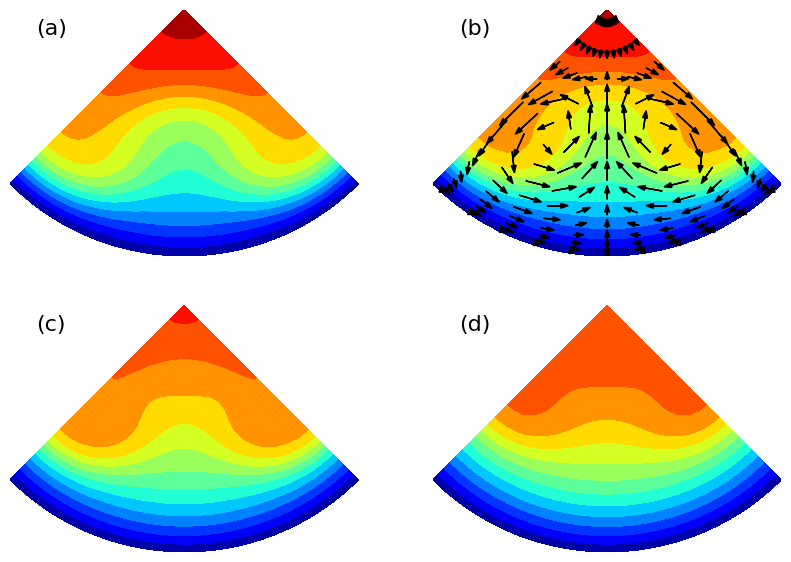
\includegraphics[width=1\linewidth]{VEL_cs.png}}
\caption{Среднее поле скорости $\V$: ряд (a) --- поперечная компонента, ряд~(b)~--- изолинии продольной компоненты, построенные с шагом $\approx 0.09$. На стенке скорость жидкости равна нулю. Изображено три сечения трубы, $x = 0, 2.5, 5$.}
% d = 0.086
\label{VEL_cs_pic}
\end{figure}

На Рисунке \ref{VEL_cs_pic} приведены поперечная $(V_r, V_\theta)$ и продольная $V_x$ компоненты стационарного течения в области, где пульсации имеют существенную амплитуду. Стационарное поперечное течение соответствует существованию в потоке стационарных продольных вихрей, поддерживающих существование полос. Там, где стационарное поперечное движение направлено от стенки к оси трубы, находятся полосы замедления. Там, где поперечное движение направлено к стенки --- полосы ускорения. 

Формирующиеся в области небольшой протяженности полосчатые структуры переносятся в переднюю и заднюю часть порыва за счет конвекции. На Рисунке \ref{V3D_cs_pic} на линии 1 средняя продольная скорости $V_x$ в системе отсчета, связанной с порывом, равна нулю. В приосевой области, ограниченной этой линией, скорость положительна, а в периферийной --- отрицательна. Видно, что полосчатые структуры во всех сечениях (кроме переднего, x = 5) располагаются в области отрицательной относительной скорости. Среднее течение с отрицательной скоростью переносит полосчатые структуры в заднюю часть порыва, где они формируют картину, похожую на вытянутые щупальца медузы (смотри Рисунок \ref{3D_img}). При $x > 5$ полосчатые структуры концентрируются в приосевой части трубы и конвектируются вперед положительной скоростью относительного движения, благодаря чему в передней части порыва $A_{3D}$ сохраняет заметную величину, несмотря на отсутствие поперечного движения.


\section{Механизм возбуждения пульсаций}

\begin{figure}
\center{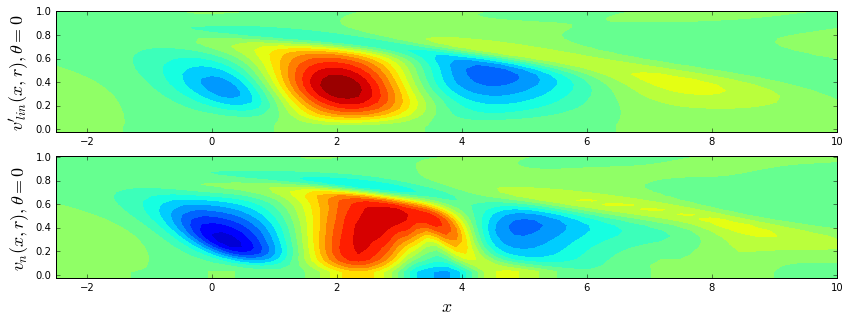
\includegraphics[width=1\linewidth]{lin_ls_cmp.png}}
\caption{Сравнение мгновенного поля продольной скорости пульсаций, возникающих в рамках линеаризованных уравнений, $\v'_1$ (a) и пульсационной составляющей движения $\v_n$ (b) в сечении $\theta = 0$. Сплошные изолинии --- положительные значения, прерывистые --- отрицательные.}
% 
\label{lin_ls_cmp_pic}
\end{figure}

Полосчатые структуры достигают максимальной амплитуды в области $x\in[-5,0]$, где создаются условия для возникновения колебаний. Наиболее вероятный механизм генерации колебаний --- механизм потери устойчивости стационарной составляющей течения. Для проверки этой гипотезы стационарное течение $\V$ было исследовано на устойчивость к малым возмущениям $\v'$. Предположение малости $\v'$ позволяет линеаризовать уравнения. Линеаризованные относительно $\v'$ уравнения Навье-Стокса в подвижной системе координат, связанной с порывом, имеют вид:
\begin{equation} \label{lin_eq}
\frac{\partial \v'}{\partial t} = c \frac{\partial \v'}{\partial x} - (\V \cdot \nabla) \v' - (\v' \cdot \nabla) \V - \nabla p' + \nu \nabla^2 \v'. 
\end{equation}
Здесь $p'$ -- пульсационная составляющая давления. Расход $\v'$ равен нулю. Другие уравнения в постановке задачи линейные и для $\v'$ имеют тот же вид, что и для $\v$. Задача решается с дополнительными условия симметрии \eqref{sym_eq}, \eqref{per_eq}, которым удовлетворяет поле скорости модельного порыва. Подчеркнем, что поле скорости $\V$ является существенно трехмерным и все три его компоненты $V_x$, $V_r$ и $V_\theta$ отличны от нуля. Хотя значения $V_r$ и $V_\theta$ на порядок ниже значения $V_x$, в главе \ref{OXgen_ch} будет показано, что их учет необходим для адекватного описания механизма поддержания продольных вихрей. Исследование на устойчивость такого поля скорости $\V$ выполнено численно. 

Линеаризованные относительно возмущений уравнения с некоторыми случайными начальными условиями интегрировались по времени до выхода решения на режим экспоненциального изменения. Обнаружено, что действительно поле скорости $\V$ неустойчиво к малым возмущениям. Растущее возмущение $\v'_1 \sim e^{(\lambda+i\omega)t}$ имеет инкремент нарастания $\lambda=0.012$ и частоту $\omega=0.116$, близкую к частоте колебаний $2\pi/60=0.105$ в решении на сепаратрисе. Что более существенно, поле скорости растущего решения $\v'_1$ качественно повторяет основные особенности поля скорости пульсационной составляющей движения модельного порыва $\v_n$. В качестве подтверждения на Рисунке \ref{lin_ls_cmp_pic} представлены мгновенные поля скорости $\v'_1$ и $\v_n$ в продольном сечении $\theta = 0$. Моменты времени подобраны так, что фазы решений совпадают. Также на Рисунке \ref{lin_amp_cmp_pic} для сравнения представлены амплитуды $\v_1'$ и $\v_n$ в нескольких сечениях трубы. Нет сомнений, что колебания возникают в результате линейной неустойчивости стационарной составляющей движения. Решение линейной задачи обладает дополнительной симметрией отражения относительно плоскости $\theta = \pi/4$, выражаемой формулой:
\begin{equation} \label{dop_sym_eq}
(-v_x, -v_r, v_\theta)(x, r, \pi/4 + \theta, t) = (v_x, v_r, v_\theta)(x, r, \pi/4 - \theta, t). 
\end{equation} 
В целом, поле $\v'_1$ имеет более простую форму, чем $\v_n$. В частности, $\v'_1$ меняется во времени по гармоническому закону. Простота формы $\v'_1$ делает его предпочтительным объектом при исследовании механизмов влияния пульсаций на среднее течение. 


\begin{figure}
\center{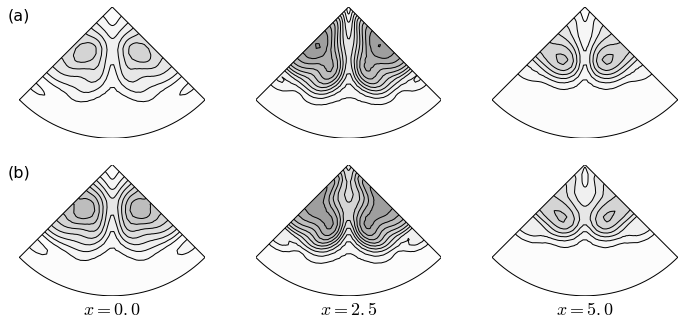
\includegraphics[width=1\linewidth]{lin_amp_cmp.png}}
\caption{Сравнение амплитуды пульсаций, возникающих в рамках линеаризованных уравнений, $\v'_1$ (ряд (a)) и пульсационной составляющей движения $\v_n$ (ряд (b)) в нескольких сечения трубы, $x = 0, 2.5, 5$. Вблизи стенки амплитуда пульсаций близка к нулю.}
\label{lin_amp_cmp_pic}
\end{figure}

В реальном течении пульсационная составляющая движения имеет конечную амплитуду и нелинейными слагаемыми в уравнении, описывающем эволюцию пульсаций, уже нельзя пренебрегать. По-видимому, роль нелинейных слагаемых сводится к тому, что они несколько меняют форму пульсаций так, что рост амплитуды пульсационной составляющей движения прекращается. При этом, именно линейные слагаемые определяют форму пульсаций и ответственны за передачу энергии в пульсационную составляющую движения. 

Отметим, что точки максимального роста колебаний находятся на линии, соответствующей нулевой относительной скорости (линия 1 на Рисунке~\ref{puls_cs_pic}). По этой причине область порождения колебаний остается неподвижной относительно порыва. Интересно, что в этой же области ($x = 0,\ r \approx 0.4$) происходит смена знака радиальной компоненты осесимметричной составляющей скорости (смотри Рисунок~\ref{U2D_pic}(b)). При $x<0$ радиальная скорость положительна, поэтому колебания, возникшие в задней части порыва, относятся в сторону стенки трубы, где относительная скорость отрицательна, и продолжают двигаться вверх по течению. Наоборот, при $x>0$ радиальная скорость направлена к оси трубы. Туда же, в область положительной скорости, сносятся и колебания, обнаруживающиеся в передней части порыва.

Отметим также, что неустойчивость полосчатых структур является неотъемлемой составляющей всех сценариев самоподдержания турбулентности в пристенных течениях. В некоторых работах предполагается, что неустойчивость возникает в пристенных областях полос замедленного движения, где в локальном профиле скорости $V_x(r)$ на фоне наибольшего градиента появляется точка перегиба --- источник неустойчивости в механизме типа Кельвина--Гельмгольца. В частности, именно такой механизм предлагается в качестве механизма возникновения колебаний в турбулентном порыве в \cite{Shimizu2009}. В рассматриваемом нами решении на сепаратрисе это определенно не так. Как видно на Рисунке~\ref{puls_cs_pic} в сечении $x=0$, соответствующем максимальной скорости роста колебаний, амплитуда колебаний минимальна как раз в области полосы замедления ($\theta=\pi/4$). Наибольшие колебания развиваются наоборот вблизи полос ускорения, а если быть более точным, в промежуточных областях между полосами. В этих областях стационарная составляющая скорости течения претерпевает наибольшее изменение и имеет точки перегиба, но не как функция радиальной переменной, а как функция угла.



\section{Влияние продольной неоднородности стационарной составляющей движения на форму пульсаций}

Замечено, что в модельном порыве область наибольшей интенсивности пульсаций совпадает с областью резкого падения скорости на его заднем фронте (смотри Рисунок \ref{ucl_cmp_img}, \ref{amp_pic}). Аналогичная особенность отмечена в турбулентном порыве \cite{Hof2010}. Чтобы оценить роль продольной неоднородности среднего течения в процессе формирования пульсаций, в работе выполнен анализ устойчивости однородных вдоль трубы полей скорости $\U_i = \V\big|_{x=x_i}$, повторяющих среднее поле скорости модельного порыва $\V$ в сечениях трубы $x = x_i$. Значения $x_i$, при которых было выполнено исследование поля скорости $\U_i$, принадлежат интервалу $(-8,4)$, где пульсационная составляющая движения получает энергию от среднего течения и имеет существенную амплитуду. Поля скорости $\U_i$ имеют полосчатую структуру и воспроизводят неоднородность среднего поля скорости по координатам $r$ и $\theta$, но теряют неоднородность среднего течения по координате $x$. Сравнение характеристик устойчивости полей скорости $\V$ и $\U_i$ позволяет делать выводы о роли продольной неоднородности в процессе формирования пульсаций. 

Собственные решения линейной задачи устойчивости однородного вдоль трубы поля скорости имеют вид $\v' = \mathrm{Real}\left(\hat \v (r, \theta, t) e^{i \alpha x}\right)$, где функция $\hat \v$ имеет комплексные значения, функция $\mathrm{Real}(z)$ имеет значение действительной части комплексного числа $z$. Постановка задачи линейной устойчивости однородного вдоль трубы поля скорости формулируется относительно $\hat \v$ и является двумерной (пропадает зависимость от $x$). Задача имеет дополнительный параметр $\alpha > 0$, характеризующий волновое число возмущения, устойчивость к которому анализируется. В этой постановке уравнения движения в системе координат, перемещающейся вдоль трубы со скоростью $c$, и уравнение неразрывности имеют вид: 
\begin{equation} \label{hat_NS_eq}
\frac{\partial \hat \v}{\partial t} = i \alpha  c \hat \v - (\U_i \cdot \hat \nabla) \hat \v - (\hat \v \cdot \nabla) \U_i - \hat \nabla \hat p + \nu \hat \nabla^2 \hat \v,
\end{equation}
\begin{equation} \label{hat_div_eq}
\hat \nabla \cdot \hat \v = 0,
\end{equation}
где функция $\hat p = \hat p(r,\theta,t)$ имеет комплексные значения, $p' = \mathrm{Real}\left(\hat p e^{i \alpha x}\right)$ --- пульсационная составляющая давления, оператор $\hat \nabla$ имеет вид: 
\begin{equation*}
\hat \nabla = \left( i\alpha, \frac{\partial}{\partial r}, \frac{\partial}{r \partial \theta} \right).
\end{equation*}
На стенках трубы ставится условие прилипания. На решение накладываются дополнительные условия симметрии \eqref{sym_eq}, \eqref{per_eq}, при которых найден модельный порыва. Условие периодичности вдоль потока \eqref{bc2_eq} снимается. 

\begin{figure}
\center{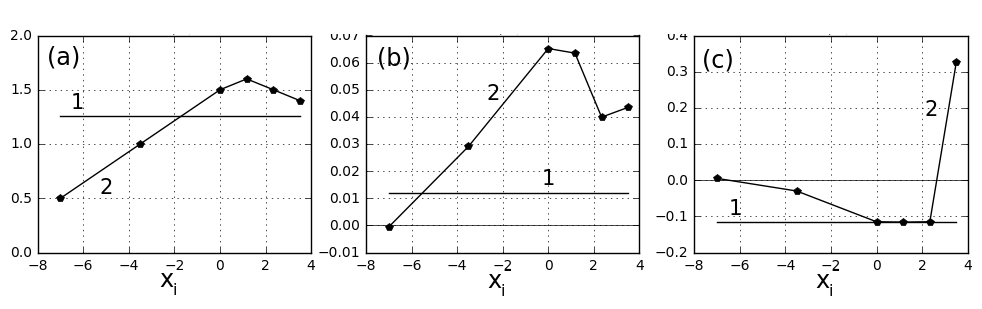
\includegraphics[width=1\linewidth]{cs_lin.png}}
\caption{Значение волнового числа $\alpha$ (a), инкремента нарастания $\lambda$ (b) и угловой частоты $\omega$ (в системе отсчета порыва) (c) для наиболее быстро растущего возмущения поля скорости модельного порыва $\V$ (линия 1) и однородных вдоль потока полей скорости $\U_i$, повторяющих $\V$ в сечении $x = x_i$ (точки на линии 2).}
\label{cs_lin_pic}
\end{figure}

На устойчивость исследованы поля скорости $\U_i = \V\big|_{x=x_i}$ для $x_i = -7.1,$ $-3.5, 0, 1.2, 2.3, 3.5$.  Для каждого исследованного $\U_i$ среди собственных решений линейной задачи устойчивости с различными значениями волнового числа $\alpha >0$ найдено наиболее быстро растущее (медленно затухающее). Наиболее быстро растущее (медленно затухающее) собственное решение линейной задачи устойчивости поля скорости $\U_i$ при фиксированном значении $\alpha$ получено интегрированием уравнений \eqref{hat_NS_eq}, \eqref{hat_div_eq} со случайными начальными данными до выхода на экспоненциальный режим роста, $||\hat \v|| \sim e^{(\lambda + i\omega) t}$. 

На Рисунке \ref{cs_lin_pic} приведены полученные значения волнового числа $\alpha$, инкремента нарастания $\lambda$ и угловой частоты $\omega$ для наиболее быстро растущих (медленно затухающих) возмущений поля скорости $\U_i$, как функции $x_i$ (точки на линии 2). Также на рисунке (линией 1) приведены характеристики наиболее быстро растущего возмущения стационарной составляющей поля скорости модельного порыва $\V$ (значение длины волны приблизительное). Угловая частота приведена в системе отсчета, перемещающейся со скоростью порыва. 

Поля скорости $\U_i$ при $x_i \in (-4,4)$ оказываются неустойчивыми, причем скорость роста наиболее быстро растущего возмущения оказывается выше скорости роста возмущений стационарной составляющей движения модельного порыва $\V$. Наибольшей скоростью роста обладают возмущения полей скорости $\U_i$ при $x_i \in (0, 2)$. Следствием этого факта может быть то, что именно при $x \in (0,2)$ пульсационная составляющая движения $\v_n$ достигает наибольшей амплитуды (смотри Рисунок \ref{amp_pic}). Наиболее быстро растущие  возмущения полей скорости $\U_i$ при $x_i \in (0,3)$ повторяют форму пульсационной составляющей движения модельного порыва. В частности, их волновые числа и угловые частоты близки к соответствующим значениям как для наиболее быстро растущих возмущений поля скорости $\V$, так и для пульсационной составляющей движения модельного порыва $\v_n$. Распределения по сечению трубы амплитуды колебаний для наиболее быстро растущих возмущений полей скорости $\U_i$ при $x_i \in (0,3)$, приведенные на Рисунке \ref{cs_lin_map_pic}, повторяют распределение амплитуды колебаний в модельном порыве (смотри Рисунок \ref{puls_cs_pic}).


\begin{figure}
\center{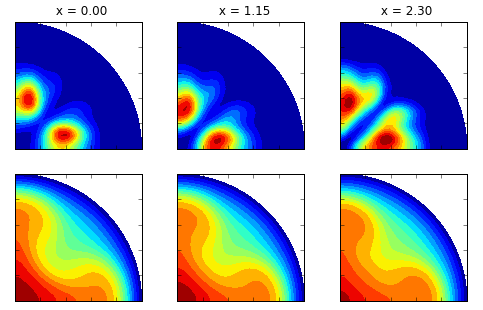
\includegraphics[width=1\linewidth]{cs_lin_map.png}}
\caption{Изолинии амплитуды колебаний для наиболее быстро растущего возмущения однородного вдоль трубы поля скорости $\U_i$ (a) и изолинии продольной компоненты поля скорости $\U_i$ (b), $x_i = 0, 1.2, 2.3$.}
\label{cs_lin_map_pic}
\end{figure}

Если при $x_i \in (0,3)$ наиболее быстро растущее возмущения полей скорости $\U_i$ повторяют качественные особенности пульсационной составляющей движения модельного порыва, то уже при $x_i = 3.5$ наиболее быстрорастущим оказывается возмущение принципиально другой формы. С этим, в частности, связано резкое отличие значения угловой частоты $\omega$, полученного при $x_i = 3.5$, от значений, полученных при меньших $x_i$ (смотри Рисунок \ref{cs_lin_pic}). 

Среди исследованных однородных вдоль трубы полей скорости, имеющих полосчатую структур, найдены неустойчивые, для которых наиболее быстрорастущие возмущения воспроизводят как качественные, так и количественные характеристики пульсационной составляющей движения модельного порыва и имеют даже большую скорость роста, чем наиболее быстрорастущие возмущение средней составляющей движения модельного порыва. Таким образом, может быть сделан вывод, что продольная неоднородность стационарной составляющей движения не является необходимым условием для возникновения пульсаций. Образование пульсаций связано с неоднородностью стационарной составляющей движения в поперечной плоскости. 


\section{Взаимодействие между компонентами движения модельного порыва}

В предыдущих разделах были выделены компоненты движения модельного порыва и основные механизмы взаимодействия между ними. Компоненты движения находятся в динамическом равновесии, поддерживая существование друг друга и, следовательно, самого порыва. Более строго обосновать полученные результаты позволяет анализ баланса кинетической энергии в системе. Вклад каждой из компонент движения в производство кинетической энергии других компонент движения может быть вычислен на основе уравнений движения, и, в зависимости от его величины, могут быть сделаны выводы о положительном или отрицательном влиянии одних компонент движения на другие. 

Ниже приведен вывод уравнений баланса кинетической энергии для каждой компоненты движения. 
Осреднение уравнения Навье-Стокса по времени в системе отсчета, связанной с порывом, дает уравнение баланса импульса стационарной составляющей движения $\V = \overline{\v}^t$:
\begin{equation} \label{VEL_eq}
\pd{\V}{t} = c \pd{\V}{x} - (\V \cdot \nabla) \V - \overline{(\v_n \cdot \nabla) \v_n}^t - \nabla P + \nu \nabla^2 \V.
\end{equation}
Здесь $c$ --- скорость перемещения порыва, $P$ --- стационарная составляющая давления, $\v_n$ --- пульсационная составляющая скорости, черта над выражением с индексом $t$ обозначает осреднение по времени. Формально производная по времени от стационарной составляющей движения равна нулю, однако слагаемое $\partial \V/ \partial t$ сохранено в записи уравнения \eqref{VEL_eq} для удобства восприятия. В сравнении с уравнением Навье-Стокса в \eqref{VEL_eq} возникает новое слагаемое $-\overline{(\v_n, \nabla) \v_n}^t$, выражающее влияние пульсационной составляющей движения на среднее течение. 

Последующее осреднение \eqref{VEL_eq} по угловой координате дает уравнения баланса импульса двумерной компоненты движения $\V_{2D} = \overline{\V}^\theta$:
\begin{multline} \label{V2D_eq}
\pd{\V_{2D}}{t} = c \pd{\V_{2D}}{x} - (\V_{2D} \cdot \nabla) \V_{2D} - \overline{(\V_{3D} \cdot \nabla) \V_{3D}}^{\theta} - \overline{(\v_n \cdot \nabla) \v_n}^{t,\theta} - \\ - \nabla P_{2D} + \nu \nabla^2 \V_{2D}.
\end{multline}
Здесь $P_{2D} = \overline{P}^{\theta}$ --- двумерная составляющая давления, $\V_{3D} = \V - \V_{2D}$ --- трехмерная составляющая скорости, черта над выражением с индексом $\theta$ --- осреднение по угловой переменной. Вычитание \eqref{V2D_eq} из \eqref{VEL_eq} дает уравнение баланса импульса трехмерной составляющей движения $\V_{3D}$:
\begin{multline} \label{V3D_eq}
\pd{\V_{3D}}{t} = c \pd{\V_{3D}}{x} - (\V_{3D} \cdot \nabla) \V_{3D} - (\V_{3D} \cdot \nabla) \V_{2D} - (\V_{2D} \cdot \nabla) \V_{3D} + \\ + \overline{(\V_{3D} \cdot \nabla) \V_{3D}}^{\theta} - \overline{(\v_n \cdot \nabla) \v_n}^{t} + \overline{(\v_n \cdot \nabla) \v_n}^{t, \theta} - \nabla P_{3D} + \nu \nabla^2 \V_{3D}.
\end{multline}
Здесь $P_{3D} = P - P_{2D}$ --- трехмерная составляющая давления. Проецирование уравнения \eqref{V3D_eq} на ось $x$ дает уравнение, описывающее баланс импульса составляющей движения $\V_S = (V_{x,3D}, 0, 0)$, ассоциированной с полосами повышенной и пониженной скорости. Проецирование уравнения \eqref{V3D_eq} на поперечное сечение трубы дает уравнение баланса импульса составляющей движения $\V_V = (0, V_{r,3D}, V_{\theta,3D})$, ассоциированной с продольными вихрями. 
%Стоит отметить, что $\V_{2D}, \V_{3D}, \v_n$ удовлетворяют условию несжимаемости \eqref{eq0_Re}, в то время как $\V_S$ и $\V_V$ не удовлетворяют ему. 

\begin{figure}
\center{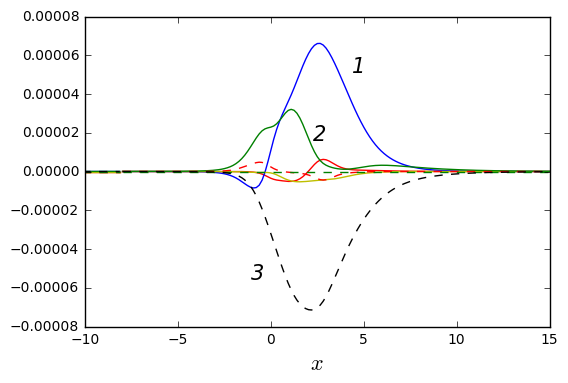
\includegraphics[width=0.6\linewidth]{e1_parts.png}}
\caption{Вклад в производство кинетической энергии пульсационной составляющей движения со стороны: 1 --- $\V_S$; 2 --- $\V_{2D}$; 3 --- вязких слагаемых. Другие слагаемые существенного вклада не дают.}
\label{e1_parts_pic}
\end{figure}

Вычитание \eqref{VEL_eq} из \eqref{NS_eq} дает уравнение эволюции пульсационной составляющей движения $\v_n$: 
\begin{multline} \label{vel1_eq}
\pd{\v_n}{t} = c \pd{\v_n}{x} - (\v_n \cdot \nabla) \v_n + \overline{(\v_n \cdot \nabla) \v_n}^t - (\V_{2D} \cdot \nabla) \v_n - (\V_S \cdot \nabla) \v_n - (\V_V \cdot \nabla) \v_n - \\ - (\v_n \cdot \nabla) \V_{2D} - (\v_n \cdot \nabla) \V_S - (\v_n \cdot \nabla) \V_V - \nabla p_n + \nu \nabla^2 \v_n. 
\end{multline}
Здесь $p_n = p - P$ --- пульсационная составляющая давления, среднее поле скорости представлено в виде суммы компонент движения $\V = \V_{2D} + \V_S + \V_V$, которые оказывают влияние на пульсационную составляющую движения через соответствующие нелинейные слагаемые. Осреднение по времени \eqref{vel1_eq}, умноженного на $\v_n$, дает уравнение изменения кинетической энергии пульсационной составляющей движения $e_n = \overline{\v_n^2/2}^t$: 
\begin{equation}\label{en_eq}
\pd{e_n}{t} = D_n^{2D} + D_n^{S} + D_n^{V} - \overline{\v_n (\v_n \cdot \nabla) \v_n}^t - \overline{\v_n \cdot \nabla p_n}^t + \nu \overline{\v_n \cdot \nabla^2 \v_n}^t,
\end{equation}
где слагаемые $D_n^{2D}$, $D_n^{S}$ и $D_n^{V}$ выражают генерацию $e_n$, обусловленную нелинейным взаимодействием $\v_n$ с компонентами движения $\V_{2D}$, $\V_S$ и $\V_V$, соответственно. Значения $D_n^{2D}$, $D_n^{S}$, $D_n^{V}$ вычисляются по формулам:
$$
D_n^{2D} = c \pd{e_n}{x}  - (\V_{2D} \cdot \nabla) e_n - \overline{\v_n (\v_n \cdot \nabla) }^t \V_{2D},
$$
$$
D_n^{S}  = - (\V_S \cdot \nabla) e_n - \overline{\v_n (\v_n \cdot \nabla)}^t \V_S,
$$
$$
D_n^{V} =  - (\V_V \cdot \nabla) e_n - \overline{\v_n (\v_n \cdot \nabla)}^t \V_V.
$$

На Рисунке \ref{e1_parts_pic} приведены графики усреднённых по сечению трубы слагаемых из правой части уравнения \eqref{en_eq}. Наибольший вклад в генерацию кинетической энергии пульсаций $e_n$ дает слагаемое $D_n^S$ (кривая 1), что согласуется с представлениями о возникновении пульсаций вследствие линейной неустойчивости полосчатого движения. Хотя и не определяющий, но существенный положительный вклад дает слагаемое $D_n^{2D}$ (кривая 2). Так как течение $e_n$ не меняется во времен, сумма всех слагаемых в правой части уравнения \eqref{en_eq} равна нулю. Положительный вклад в генерацию $e_n$ со стороны $D_n^S$ и $D_n^{2D}$ компенсируется вязким слагаемым (кривая 3). Влияние других слагаемых оказывается незначительным. 

\begin{figure}
\center{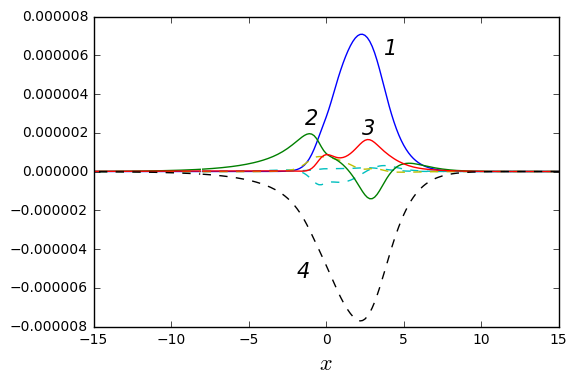
\includegraphics[width=0.6\linewidth]{ev_parts.png}}
\caption{Вклад в производство кинетической энергии движения $\V_V$, ассоциированного с продольными вихрями, со стороны: 1 --- $\v_n$; 2 --- $\V_{2D}$; 3 --- градиента давления; 4 --- вязких слагаемых. Другие слагаемые существенного вклада не дают.}
\label{ev_parts_pic}
\end{figure}

Аналогично, осреднение по $\theta$ уравнения \eqref{V3D_eq}, умноженного на поле скорости $\V_V$, ассоциированного с продольными вихрями, дает уравнение баланса кинетической энергии $E_V = \overline{\V_V^2/2}^\theta$:
\begin{equation}\label{EV_eq}
\pd{E_V}{t} = D_V^{2D} + D_V^{2D,S} + D_V^{S} + D_V^n - \overline{\V_V (\V_V \cdot \nabla) \V_V}^\theta - \overline{\V_V \nabla P_{3D}}^\theta + \nu \overline{\V_V \nabla^2 \V_V}^\theta,
\end{equation}
где слагаемые $D_V^{2D}$, $D_V^{2D,S}$, $D_V^S$, $D_V^n$ описывают влияние на поле скорости $\v_n$ компонент движения $\V_{2D}$, $\V_S$, $\V_n$, обусловленное нелинейным взаимодействие между ними. Значения $D_V^{2D}$, $D_V^{2D,S}$, $D_V^S$, $D_V^n$ вычисляются по формулам:
$$
D_V^{2D} = c \pd{E_V}{x} - (\V_{2D} \cdot \nabla) E_V - \overline{\V_V (\V_V \cdot \nabla)}^\theta \V_{2D},
$$
$$
D_V^{2D,S} = - \overline{\V_V (\V_S \cdot \nabla)}^\theta \V_{2D},
$$
$$
D_V^{S} = - \overline{\V_V (\V_S \cdot \nabla) \V_V}^\theta,
$$
$$
D_V^n = - \overline{\V_V (\v_n \cdot \nabla) \v_n}^{t,\theta}.
$$

Графики усредненных по сечению трубы слагаемых правой части уравнения \eqref{EV_eq} приведены на Рисунке \ref{ev_parts_pic}. В соответствии с общими представлениями, наибольший вклад в производство продольных вихрей дает пульсационная составляющая движения. Её вклад в образование кинетической энергии $E_V$ выражает слагаемое $D_V^n$ (линия 1). Также существенный положительный вклад дает градиент давления, однако его интегральный вклад ниже почти в $5$ раз (линия 3). Слагаемое, выражающее вклад градиента давления в производство $E_V$, отлично от нуля, так как поле скорости $\V_V$ не соленоидальное. Также можно отметить влияние $\V_{2D}$, выраженное слагаемым $D_V^{2D}$ (линия 2). При $x > 0$ оно отрицательно, а при $x < 0$ --- положительно. Такое поведение соответствует тому, что продольная завихренность, формирующейся при положительных $x$, сносится вверх по течению вместе с основным потоком вблизи стенки за счет конвекции. Производство кинетической энергии $E_V$ перечисленными слагаемыми компенсируется вязким слагаемым (линия 4). Другие слагаемые в уравнении \eqref{EV_eq} существенного влияния не оказывают. 

\begin{figure}
\center{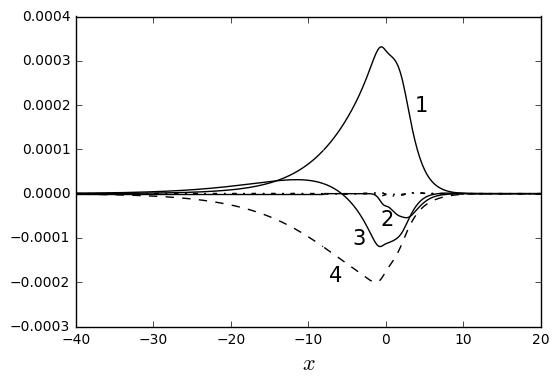
\includegraphics[width=0.6\linewidth]{es_parts.png}}
\caption{Вклад в кинетическую энергию движения $\V_S$, ассоциированного с полосами, со стороны: 1 --- $\V_V$ и $\V_{2D}$; 2 --- $\v_n$; 3 --- $\V_{2D}$; 4 --- вязких слагаемых. Другие слагаемые существенного вклада не дают.}
\label{es_parts_pic}
\end{figure}

Осреднение по переменной $\theta$ уравнения \eqref{V3D_eq}, умноженного на поле скорости $\V_S$,  ассоциированное с полосами, дает уравнение баланса кинетической энергии $E_S = \overline{\V_S^2/2}^\theta$:
\begin{equation}\label{ES_eq}
\pd{E_S}{t} = D_S^{2D} + D_S^{2D,V} + D_S^V + D_S^n - \overline{\V_S (\V_S \cdot \nabla) \V_S}^\theta - \overline{\V_S \nabla P_{3D}}^\theta + \nu \overline{\V_S \nabla^2 \V_S}^\theta.
\end{equation} 
Слагаемые $D_S^{2D}$, $D_S^{2D,V}$, $D_S^V$, $D_S^n$ вычисляются по формулам:
$$
D_S^{2D} = c \pd{E_S}{x} - (\V_{2D} \cdot \nabla) E_S - \overline{\V_S (\V_S \cdot \nabla)}^\theta \V_{2D},
$$
$$
D_S^{2D,V} = - \overline{\V_S (\V_V \cdot \nabla)}^\theta \V_{2D},
$$
$$
D_S^{V} = - \overline{\V_S (\V_V \cdot \nabla) \V_S}^\theta,
$$
$$
D_S^n = - \overline{\V_S (\v_n \cdot \nabla) \v_n}^{t,\theta}.
$$

Графики усредненных по сечению трубы слагаемых правой части уравнения \eqref{ES_eq} приведены на Рисунке \ref{es_parts_pic}. В этом случае наибольший вклад дает слагаемое $D_S^{2D,V}$ (линия 1). Оно выражает совместное влияние на $\V_S$ со стороны компонент движения $\V_{2D}$ и $\V_V$ и в скалярных переменных имеет вид:
$$
D_S^{2D,V} =  - V_{x, S} V_{r, V} \pd{V_{x, 2D}}{r}.
$$
Доминирующая роль этого слагаемого согласуется с представлением о том, что продольные вихри формируются за счет <<лифт-ап>> эффекта. Нормальной к стенке трехмерная компонента скорости $V_{r,V} = V_{r,3D}$ перераспределяет продольный импульс двумерного основного течения $V_{x, 2D}$, образуя тем самым трехмерную составляющую продольной скорости $V_{x,3D} = V_{x,S}$. Пульсации оказывают небольшое отрицательное влияние на формирование полос (линия 2). Двумерное течение оказывает отрицательное влияние вблизи нуля, в то время, как в задней части порыва, при $x \sim -10$, его влияние оказывается положительным (линия 3). По-видимому, это связанно с конвективным переносом полос, формирующихся в передней части порыва, в его заднюю часть вблизи стенки, осуществляемое основным течением $\V_{2D}$. Получаемая составляющей движения $\V_S$ энергия компенсируется вязким слагаемым (линия 4). Другие слагаемые существенного влияния не оказывают. 

Полученные в разделе результаты подтверждают существующие представления о взаимодействии между компонентами движения модельного порыва. Также полученные результаты указывают на то, что все существенные взаимодействия между компонентами движения выделены и учтены. Данные о производстве кинетической энергии двумерной компоненты движения в разделе не приведены. За поддержание двумерного течения ответственен внешний перепад давления. Производимая внешним перепадом давления кинетическая энергия компенсируется вязкими слагаемыми. 



\section{Выводы по главе}

В главе представлены результаты численного исследования модельного порыва. Соответствующее модельному порыву решение уравнений Навье-Стокса является предельным состоянием решения, эволюционирующего на сепаратрисе, разделяющей в фазовом пространстве области притяжения решений, соответствующих ламинарному и турбулентному режимам течения. Предельное решение на сепаратрисе описывает локализованную в пространстве структуру, перемещающуюся вниз по потоку с постоянной скоростью. В сопутствующей системе отсчета при наложенных условиях симметрии оно оказывается периодическим по времени. Модельный порыв воспроизводит некоторые характерные особенности турбулентного порыва, а простота временного поведения позволяет выполнить его подробное исследование. Мы полагаем, что исследование модельного порыва может помочь приблизиться к пониманию турбулентного порыва.

При изучении модельного порыва установлены его основные характеристики, такие как скорость перемещения вдоль трубы и период изменения во времени. Составлено представление о его внутренней структуре и выделены основные элементы цикла поддержания колебаний. Осреднение по времени в сопутствующей системе отсчета позволило разделить поле скорости модельного порыва на среднюю и пульсационную составляющие. Характерной особенностью среднего течения является наличие вытянутых вдоль потока полос повышенной и пониженной скорости, чередуются в угловом направлении. Показано, что пульсационная составляющая движения возникает в результате линейной неустойчивости среднего течения. Пульсации возникают в областях между соседними полосами повышенной и пониженной скорости, где распределение средней продольной скорости имеет точки перегиба, если рассматривать его как функцию угловой переменной. Вероятным механизмом образования пульсаций является неустойчивость струйного течения с точками перегиба. Изменение среднего течения вдоль оси $x$ существенного влияния на формирование пульсаций не оказывает. Показано, что полосы образуются за счет так называемого <<лифт-ап>> эффекта. В течении существуют стационарные продольные вихри, перемещающие жидкость в нормальной к основному потоку плоскости. Там, где медленная жидкость перемещается от стенки в основной поток, образуются полосы пониженной скорости. Между полосами пониженной скорости, где жидкость перемещается ближе к стенке, формируются полосы повышенной скорости. Формируясь в области небольшой протяженности, полосы вытягиваются вверх по потоку за счет конвекции. Полученные результаты позволяют сделать вывод о том, что поддержание стационарных продольных вихрей связано с наличием пульсаций. Такое представление подтверждается в следующей главе, посвященной механизму образования продольных вихрей.

Согласованность результатов, полученных на нескольких расчетных сетках, между собой и с результатами других авторов позволяет сделать вывод о том, что полученное предельное решение на сепаратрисе является решением уравнений Навье-Стокса и не зависит от выбора численного метода, которым оно было получено, и параметров расчета.

 

%[2] Kline, S. J., Reynolds, W. C., Schraub, F. A. & Runstadler, P. W. 1967 The structure of turbulent boundary layers. J. Fluid Mech. 30, 741–773.

%[19] Smith, C. R. & Metzler, S. P. 1983 The characteristics of low-speed streaks in the near-wall region of a turbulent boundary layer. J. Fluid Mech. 129, 27–54.

%[20] Kim, H. T., Kline, S. J. & Reynolds, W. C. 1971 The production of turbulence near a smooth wall in a turbulent boundary layers. J. Fluid Mech. 50, 133–160.

%[21] Hamilton, K., Kim, J. & Waleffe, F. 1995 Regeneration mechanisms of near-wall turbulence structures. J. Fluid Mech. 287, 317–348.
%[22] Jimenez, J. & Pinelli, A. 1999 The autonomous cycle of near wall turbulence. J. Fluid Mech. 389, 335–359.
%[23] Schoppa, W. & Hussain, F. 2002 Coherent structure generation in near-wall turbulence. J. Fluid Mech. 453, 57–108.
%[24] Waleffe, F. 1995 Hydrodynamic stability and turbulence: Beyond transients to a self-sustaining process. Stud. Appl. Maths 95, 319–343.
%[25] Waleffe, F. 1997 On a self-sustaining process in shear flows. Phys. Fluids 9, 883–900.











